% The network and sampler at a glance, one column wide; architecture.tex is the full diagram.
% Build with XeLaTeX (Inter is vendored in ../../fonts): xelatex schematic.tex
\documentclass[border=1pt]{standalone}
\usepackage{amsmath}
\usepackage{fontspec}
\setmainfont{Inter}[Path=../../fonts/, Extension=.ttf, UprightFont=*-Regular,
  ItalicFont=*-Italic, BoldFont=*-SemiBold]
\usepackage[italic]{mathastext}
\usepackage{tikz}
\usetikzlibrary{positioning,fit,arrows.meta,calc,backgrounds}

% style.py: ink, chrome and the categorical slots, as architecture.tex
\definecolor{ink}{HTML}{16161A}
\definecolor{ink2}{HTML}{55555C}
\definecolor{muted}{HTML}{909098}
\definecolor{axis}{HTML}{B8B8BF}
\definecolor{wash}{HTML}{F2F2F4}
\definecolor{blue}{HTML}{2A78D6}
\definecolor{orange}{HTML}{EB6834}
\definecolor{violet}{HTML}{6250D6}
\definecolor{green}{HTML}{1BAF7A}
\colorlet{xfill}{blue!12}
\colorlet{sfill}{violet!11}
\colorlet{rfill}{green!12}
\colorlet{xlane}{blue!4}

\newcommand{\sm}{\fontsize{6.3}{7.2}\selectfont}
\begin{document}
\fontsize{7}{8.4}\selectfont
\hyphenpenalty=10000
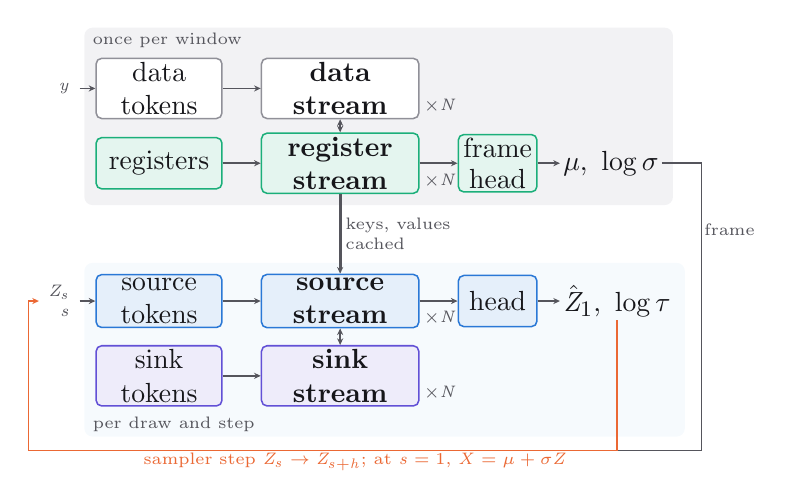
\begin{tikzpicture}[
    x=1mm, y=1mm, text=ink,
    >={Stealth[length=2.4pt,width=2.2pt]},
    box/.style={draw=#1, rounded corners=2pt, line width=0.55pt, align=center,
                inner sep=1.4pt, minimum height=6.5mm},
    xbox/.style={box=blue, fill=xfill},
    sbox/.style={box=violet, fill=sfill},
    ybox/.style={box=muted, fill=white},
    rbox/.style={box=green, fill=rfill},
    note/.style={font=\sm, text=ink2, align=center},
    arr/.style={->, line width=0.55pt, draw=ink2},
    kv/.style={->, line width=1pt, draw=ink2},
    joint/.style={<->, line width=0.5pt, draw=ink2},
    loop/.style={->, line width=0.55pt, draw=orange},
  ]
  \def\yy{27}
  \def\yr{17.5}
  \def\yx{0}
  \def\ys{-9.5}

  % one lane per stream, each with its own weights
  \foreach \s/\y/\tok/\name in {y/\yy/data tokens/data stream, r/\yr/registers/register stream,
                                x/\yx/source tokens/source stream, s/\ys/sink tokens/sink stream} {
    \node[\s box, text width=15mm, anchor=west] (\s emb) at (9, \y) {\tok};
    \node[\s box, text width=19mm, anchor=west] (\s st) at (30, \y) {\textbf{\name}};
    \draw[arr] (\s emb) -- (\s st);
    \node[note, anchor=west, inner sep=0.5pt] at ($(\s st.east)+(0.3,-2.2)$) {$\times N$};
  }

  % inputs and readouts
  \node[note, anchor=east, align=right] (sin) at (7, \yx) {$Z_s$\\ $s$};
  \draw[arr] (sin) -- (xemb);
  \node[xbox, text width=9mm, anchor=west] (shd) at (55, \yx) {head};
  \node[anchor=west, inner sep=1pt] (sout) at (68, \yx) {$\hat Z_1,\ \log\tau$};
  \draw[arr] (xst) -- (shd);
  \draw[arr] (shd) -- (sout);
  \node[note, anchor=east] (din) at (7, \yy) {$y$};
  \draw[arr] (din) -- (yemb);
  \node[rbox, text width=9mm, anchor=west] (dhd) at (55, \yr) {frame\\[-1pt] head};
  \node[anchor=west, inner sep=1pt] (dout) at (68, \yr) {$\mu,\ \log\sigma$};
  \draw[arr] (rst) -- (dhd);
  \draw[arr] (dhd) -- (dout);

  % joint attention within each pair; one-way across: cached data and register keys and values
  \draw[joint] (xst.south) -- (sst.north);
  \draw[joint] (yst.south) -- (rst.north);
  \draw[kv] (rst.south) -- node[note, right, pos=0.5, align=left, inner sep=1.5pt]
    {keys, values\\ cached} (xst.north);

  % the frame enters the source tokens and maps the last step back
  \draw[arr, -] (dout.east) -- (86, \yr) -- (86, -19) -- (sout.south |- 0,-19);
  % the sampler: one midpoint step, back to the source tokens
  \draw[loop] (sout.south) |- (0.5, -19) |- (sin.west);
  \node[note, text=orange, anchor=north, fill=white, inner sep=0.8pt] at (42, -19)
    {sampler step $Z_s\to Z_{s+h}$; at $s=1$, $X=\mu+\sigma Z$};
  \node[note, anchor=west, inner sep=0.8pt] at (86, 9) {frame};

  % lanes, behind everything
  \begin{scope}[on background layer]
    \node[fill=wash, rounded corners=3pt, inner sep=1.4mm,
          fit={(yemb) (dout) (rst) ($(yst.north)+(0,2.4)$)}] (dlane) {};
    \node[fill=xlane, rounded corners=3pt, inner sep=1.4mm,
          fit={(xemb) (sout) (sst) ($(sst.south)+(0,-2.4)$)}] (slane) {};
  \end{scope}
  \node[note, anchor=north west, inner sep=0.8pt] at ($(dlane.north west)+(0.8,-0.4)$)
    {once per window};
  \node[note, anchor=south west, inner sep=0.8pt] at ($(slane.south west)+(0.8,0.4)$)
    {per draw and step};
\end{tikzpicture}
\end{document}
